\documentclass[hyperref=unicode]{beamer}

\usepackage[absolute,overlay]{textpos}
\usepackage{graphicx}
\usepackage{adjustbox}
\usepackage{chemfig}
\usepackage[version=4]{mhchem}
\usepackage{wrapfig}
\usepackage{multirow}
\adjustboxset*{center}
\usepackage{caption}
\usepackage{chemformula}
\usepackage{elements}

%dělení slov
\usepackage{ragged2e}
\let\raggedright=\RaggedRight
%konec dělení slov

\usepackage{fontspec}
\usepackage{unicode-math}

\usepackage{polyglossia}
\setdefaultlanguage{czech}

\def\uv#1{„#1“}

\mode<presentation>{\usetheme{Madrid}}
\DefineNamedColor{named}{pozadi}{RGB}{200,200,200}
\usecolortheme{crane}

\setbeamertemplate{footline}[frame number]

\addtobeamertemplate{frametitle}{
	\let\insertframetitle\insertsectionhead}{}
\addtobeamertemplate{frametitle}{
	\let\insertframesubtitle\insertsubsectionhead}{}

\makeatletter
\CheckCommand*\beamer@checkframetitle{\@ifnextchar\bgroup\beamer@inlineframetitle{}}
\renewcommand*\beamer@checkframetitle{\global\let\beamer@frametitle\relax\@ifnextchar\bgroup\beamer@inlineframetitle{}}
\makeatother
\setbeamercolor{section in toc}{fg=blue}
\setbeamertemplate{section in toc shaded}[default][100]

\usepackage{tikz}
\usetikzlibrary{positioning}
\usetikzlibrary{arrows}
\usetikzlibrary{shapes.multipart}

\title[Crisis]
{Izomerie anorganických a organických sloučenin}
\subtitle{Polohová, funkční, koordinační a optická izomerie}
\author{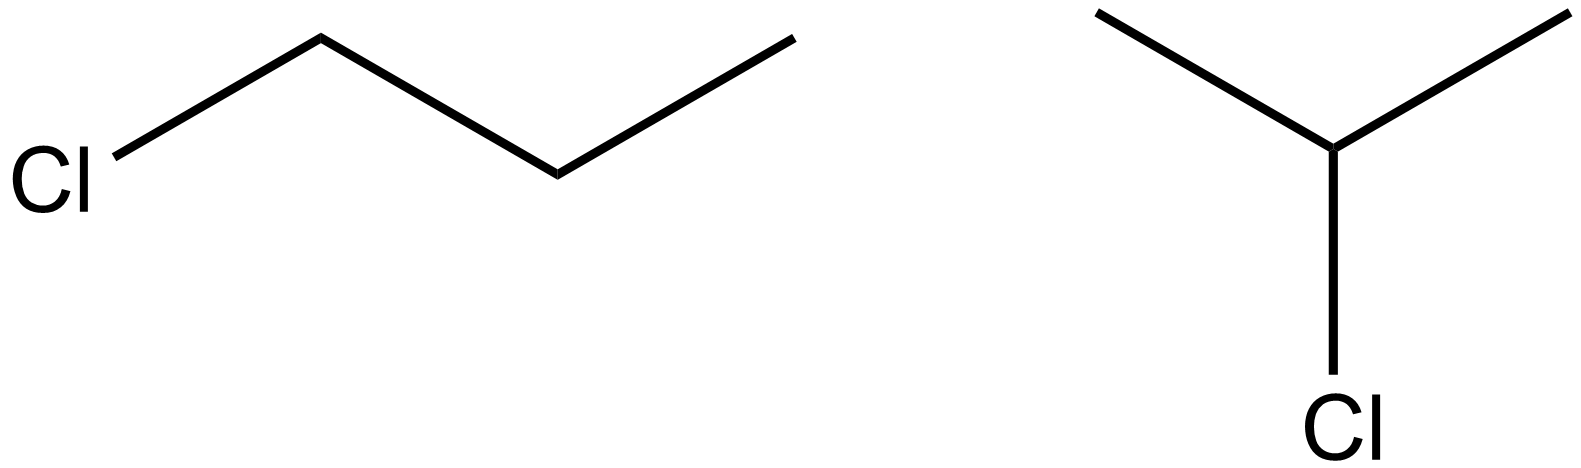
\includegraphics[keepaspectratio,width=.7\textwidth]{img/izomerie.png}}
\date{}

\begin{document}
\frame{
	\titlepage
}

\section{Izomerie}

\frame{
	\frametitle{}
	\begin{itemize}
		\item \textit{Izomerie} je vzájemný vztah dvou nebo více sloučenin, které mají stejný sumární vzorec, ale liší se uspořádáním atomů v molekule.
		\item \textit{Konstituční (strukturní)} izomery se liší polohou jednotlivých atomů v molekule:
		\item \textit{Polohové izomery} se liší polohou funkční skupiny v molekule, např. 1-chlorpropan a 2-chlorpropan:
	\end{itemize}

	\begin{figure}
		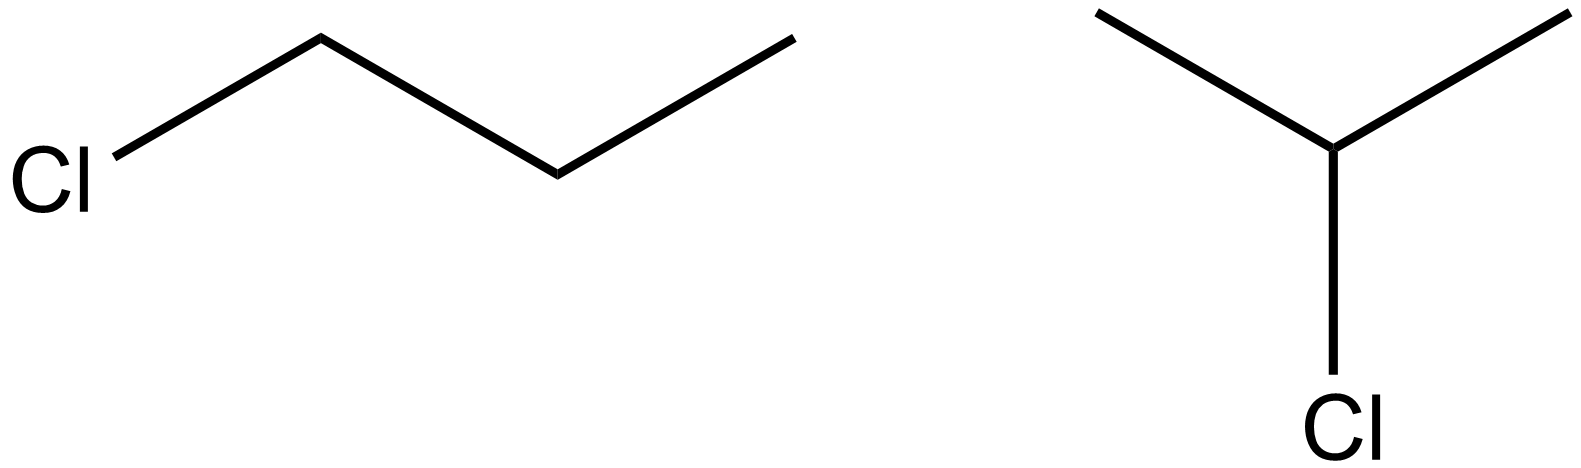
\includegraphics[width=.6\textwidth]{img/izomerie.png}
	\end{figure}

	\begin{itemize}
		\item \textit{Funkční izomery} se liší typem funkční skupiny, např. ethanol a dimethylether:
		\item \ce{CH3-CH2-OH} vs. \ce{CH3-O-CH3}
	\end{itemize}
}

\frame{
	\frametitle{}
	\begin{itemize}
		\item \textit{Tautomery} se liší polohou dvojné vazby a kyselého protonu v molekule.
		\item Příkladem je keto a enol forma acetylacetonu.
	\end{itemize}

	\begin{figure}
		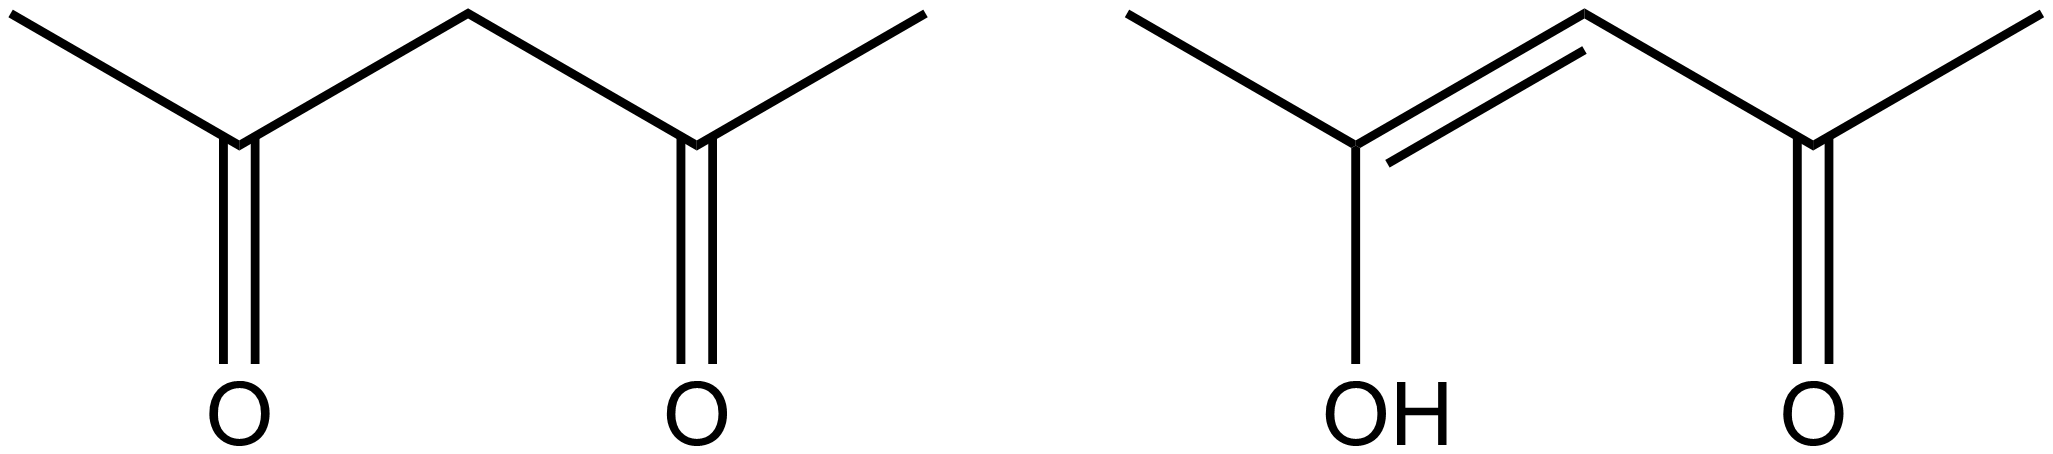
\includegraphics[width=.6\textwidth]{img/acac.png}
	\end{figure}

	\begin{itemize}
		\item \textit{Stereoizomery} mají stejnou strukturu, ale liší se prostorovou geometrii.
		\item \textit{Cis a trans izomery} se liší geometrií na násobné vazbě nebo cyklu.
	\end{itemize}
}

\frame{
	\frametitle{}
	\begin{figure}
		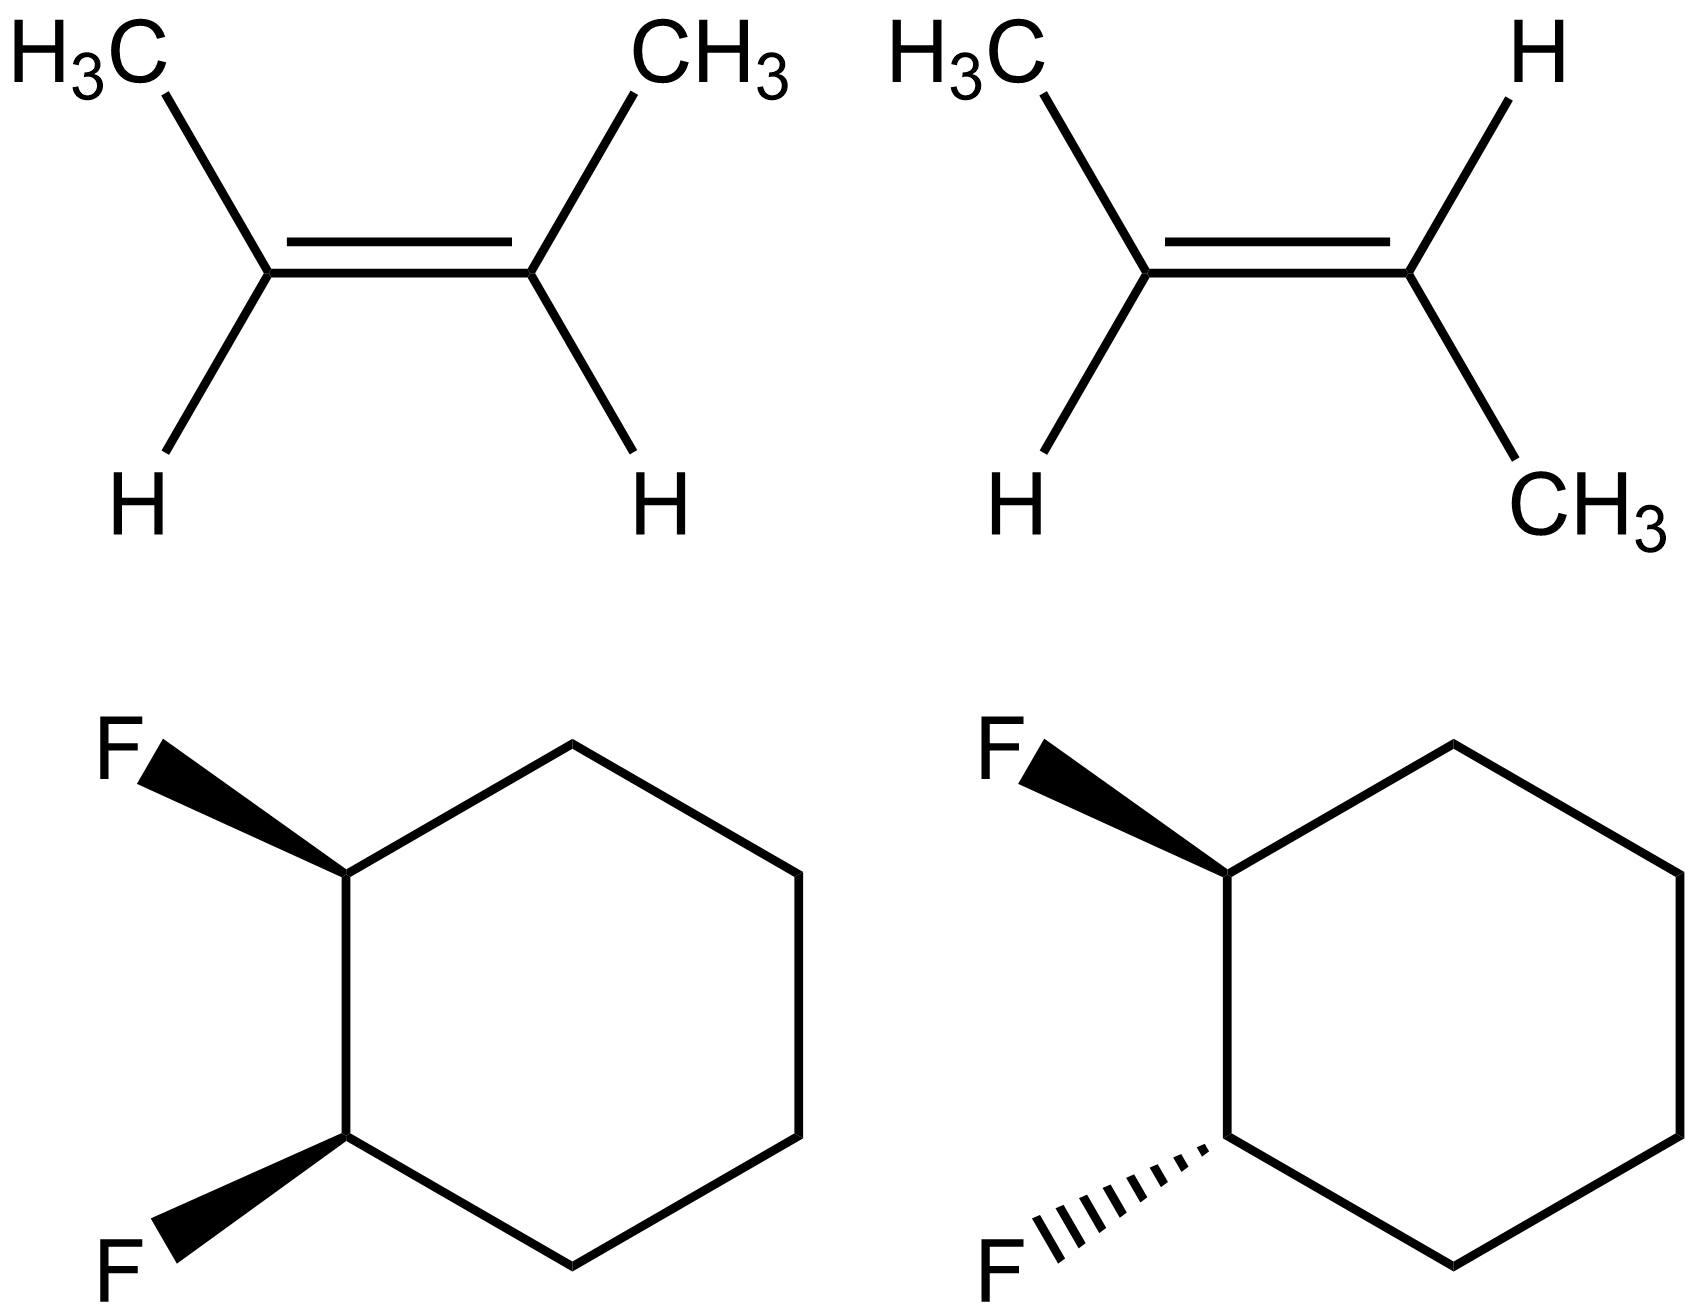
\includegraphics[width=.75\textwidth]{img/cis-trans.png}
		\caption*{Ukázky cis a trans izomerie}
	\end{figure}
}

\section{Chiralita}
\frame{
	\frametitle{}
	\begin{itemize}
		\item Chiralita označuje asymetrii prostorového rozložení objektu, např. molekuly.
		\item Chirální je objekt, který nelze ztotožnit s jeho zrcadlovým odrazem, jde např. o levotočivou a pravotočivou šroubovici.
		\item Organické chirální molekuly zpravidla obsahují uhlík se čtyřmi různými substituenty, ten označujeme jako \textit{chirální centrum}.
	\end{itemize}

	\begin{figure}
		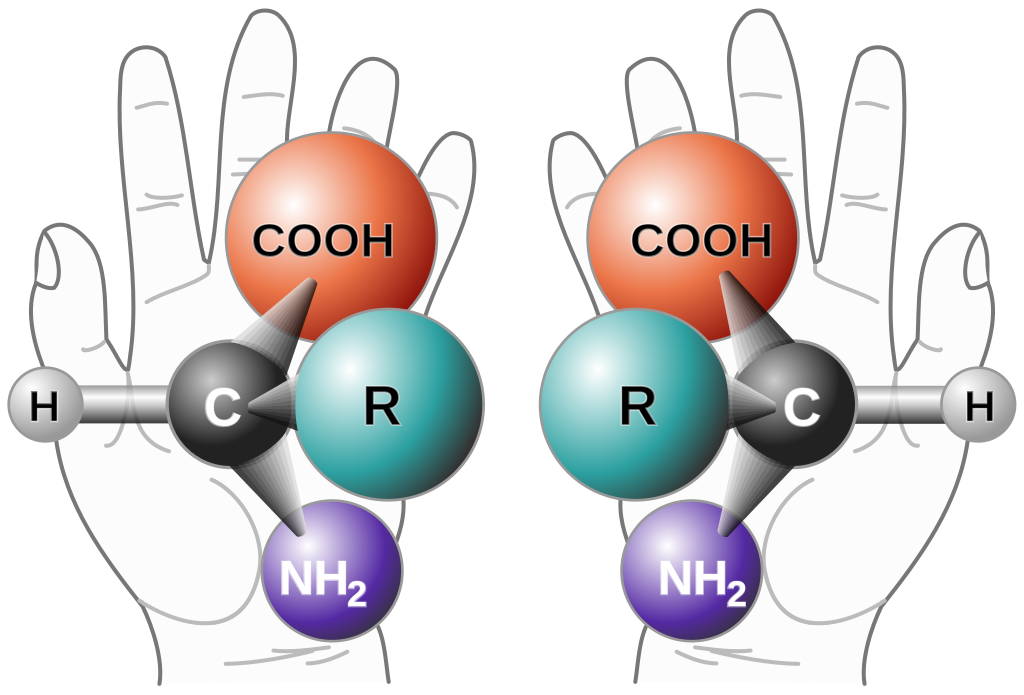
\includegraphics[width=.45\textwidth]{img/Chirality_with_hands.png}
		\caption*{Ukázka chirální molekuly.\footnote[frame]{Zdroj: \href{https://commons.wikimedia.org/wiki/File:Chirality_with_hands.svg}{Perhelion/Commons}}}
	\end{figure}
}

\frame{
	\frametitle{}
	\begin{itemize}
		\item Pokud mají izomery inverzní konfiguraci u všech chirálních center, označují se jako \textit{enantiomery}.
		\item Enantiomery mají chemické a fyzikální vlastnosti shodné, ale liší se směrem otáčení roviny polarizovaného světla (optické otáčivosti). Mohou se také lišit reaktivitou s opticky aktivními sloučeninami.
		\item Pokud má sloučenina více chirálních center a izomery se liší konfigurací pouze části z nich, označují se jako \textit{diastereomery}.
		\item Diastereomery se liší fyzikálními i chemickými vlastnostmi.
	\end{itemize}

	\begin{figure}
	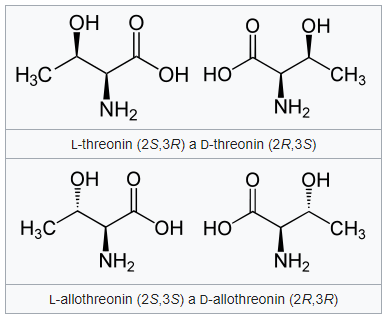
\includegraphics[width=.4\textwidth]{img/diastereomery-enantiomery.png}
\end{figure}
}

\frame{
	\frametitle{}
	\begin{columns}
		\begin{column}{.5\textwidth}
			\begin{figure}
				\scalebox{-1}[1]{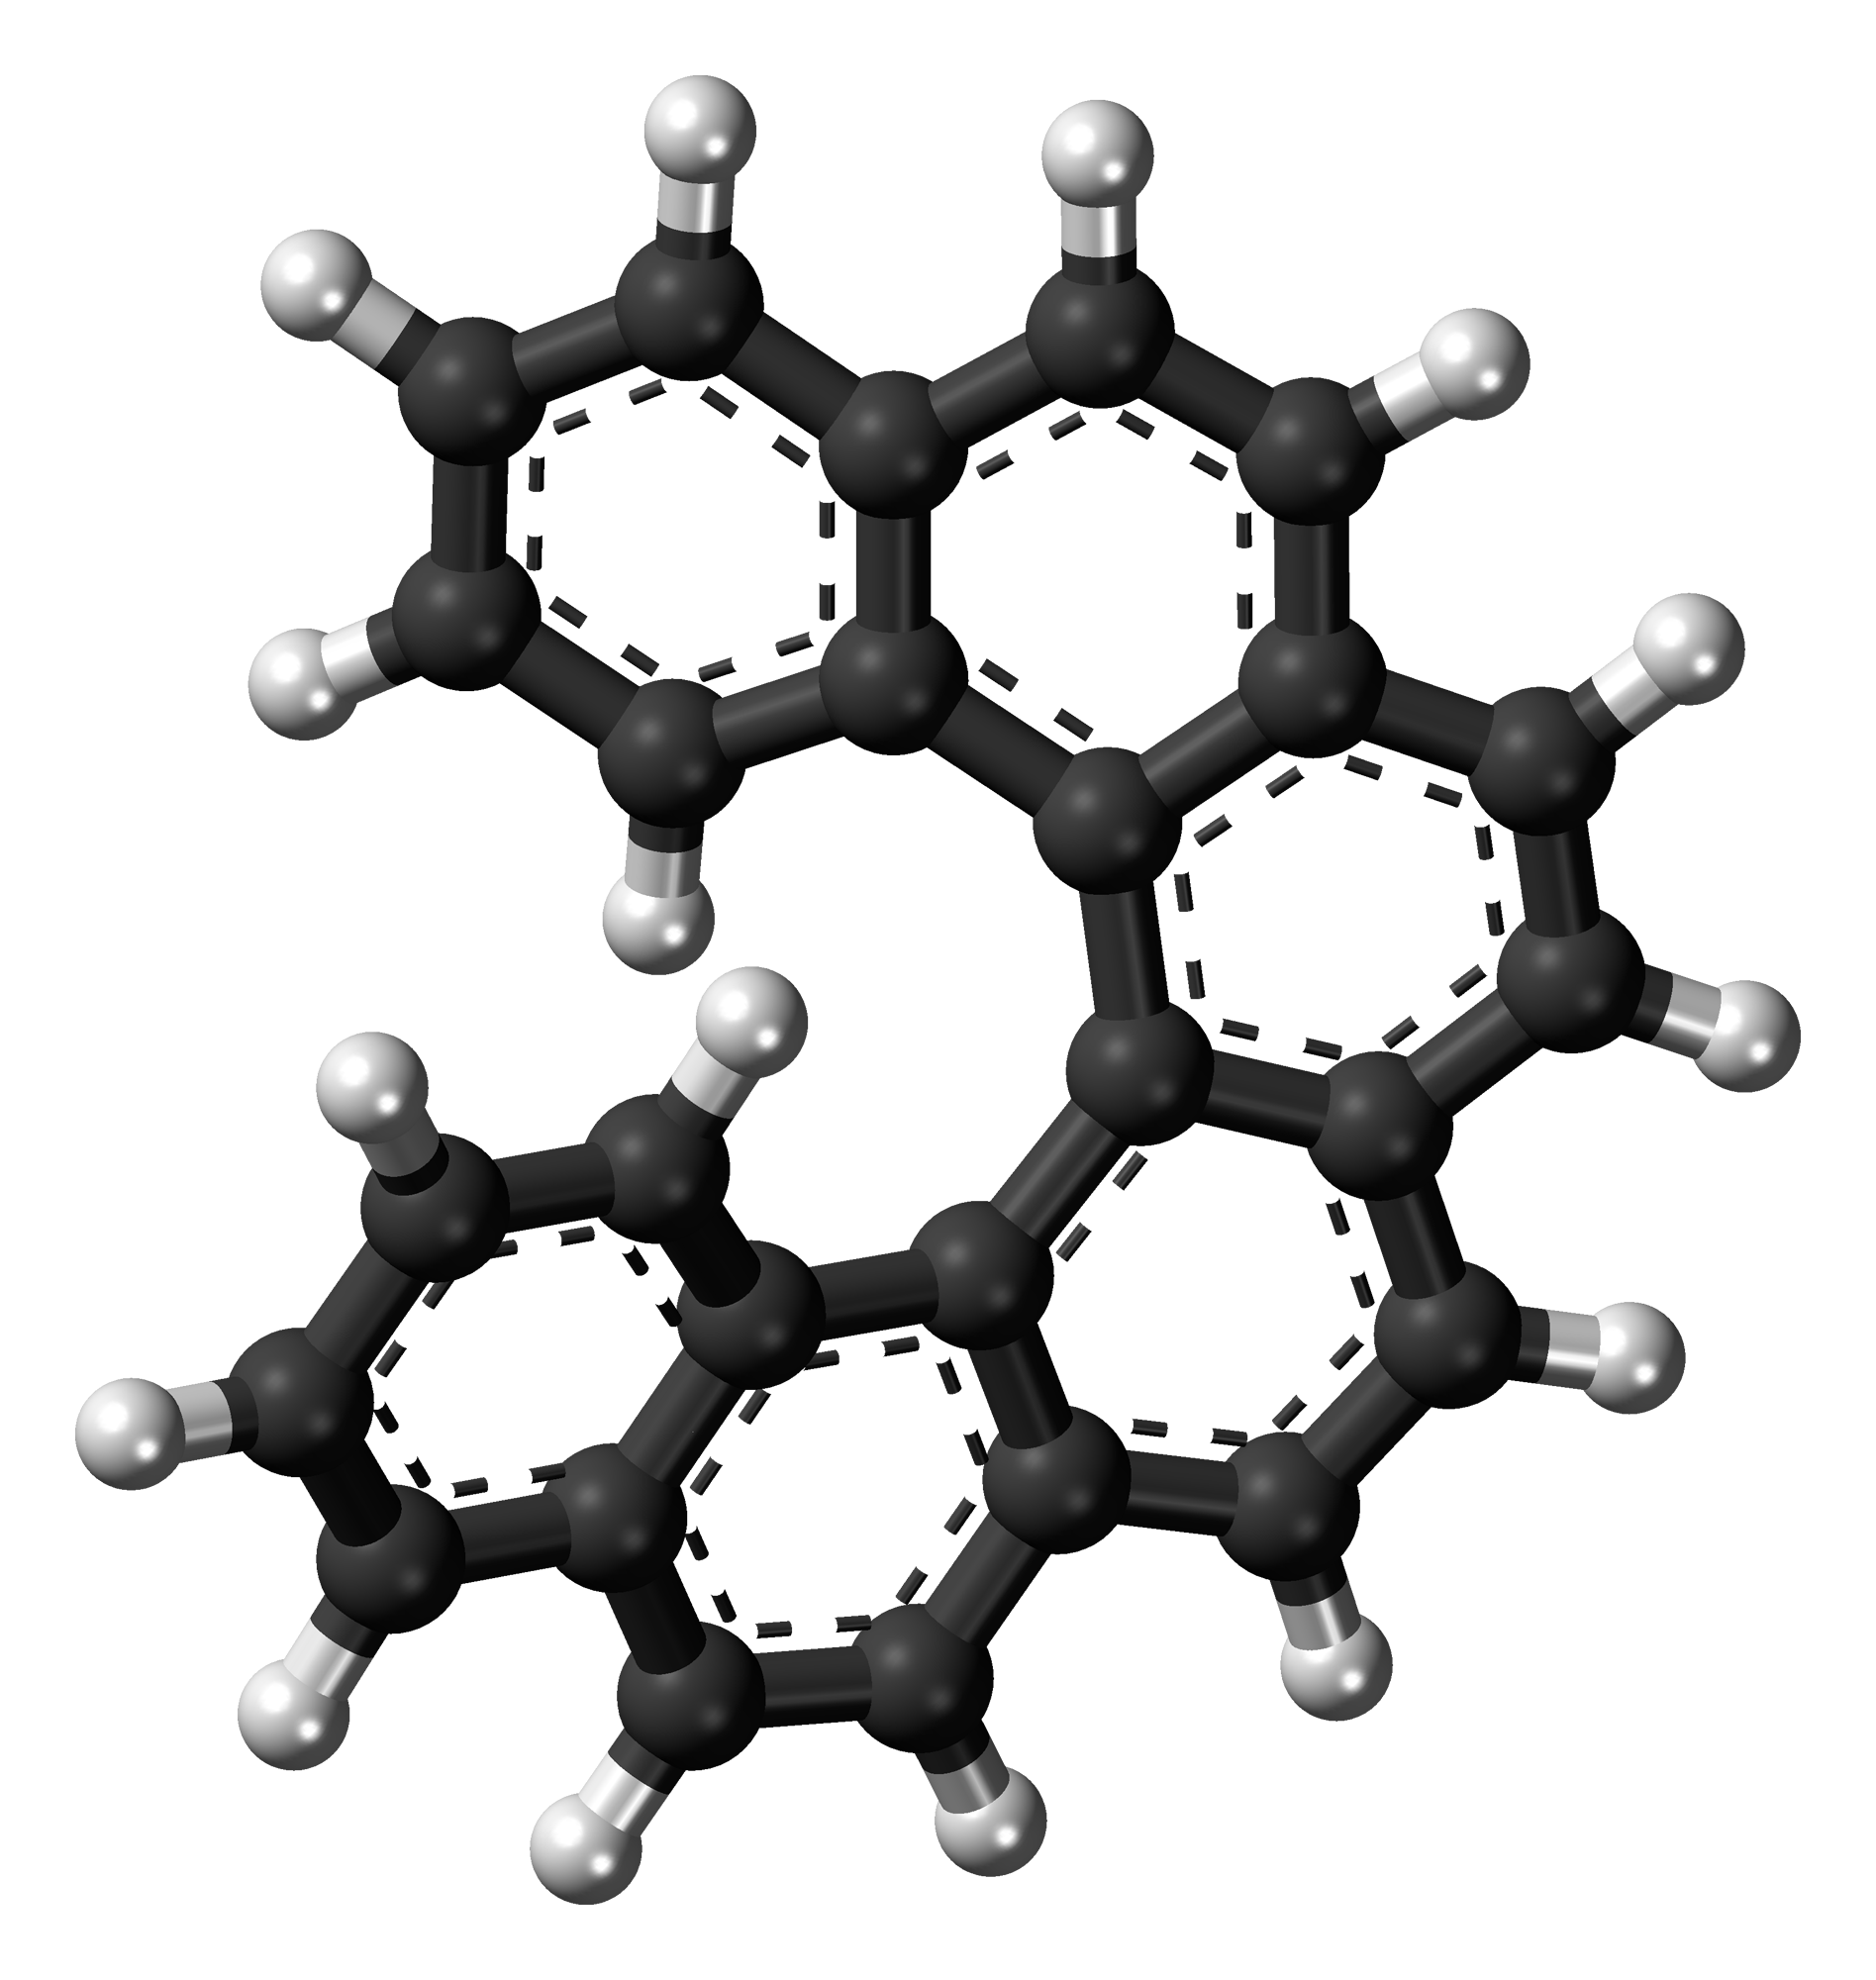
\includegraphics[height=.7\textheight]{img/Hexahelicene-3D-balls.png}}
			\end{figure}
		\end{column}
		\begin{column}{.5\textwidth}
			\begin{figure}
				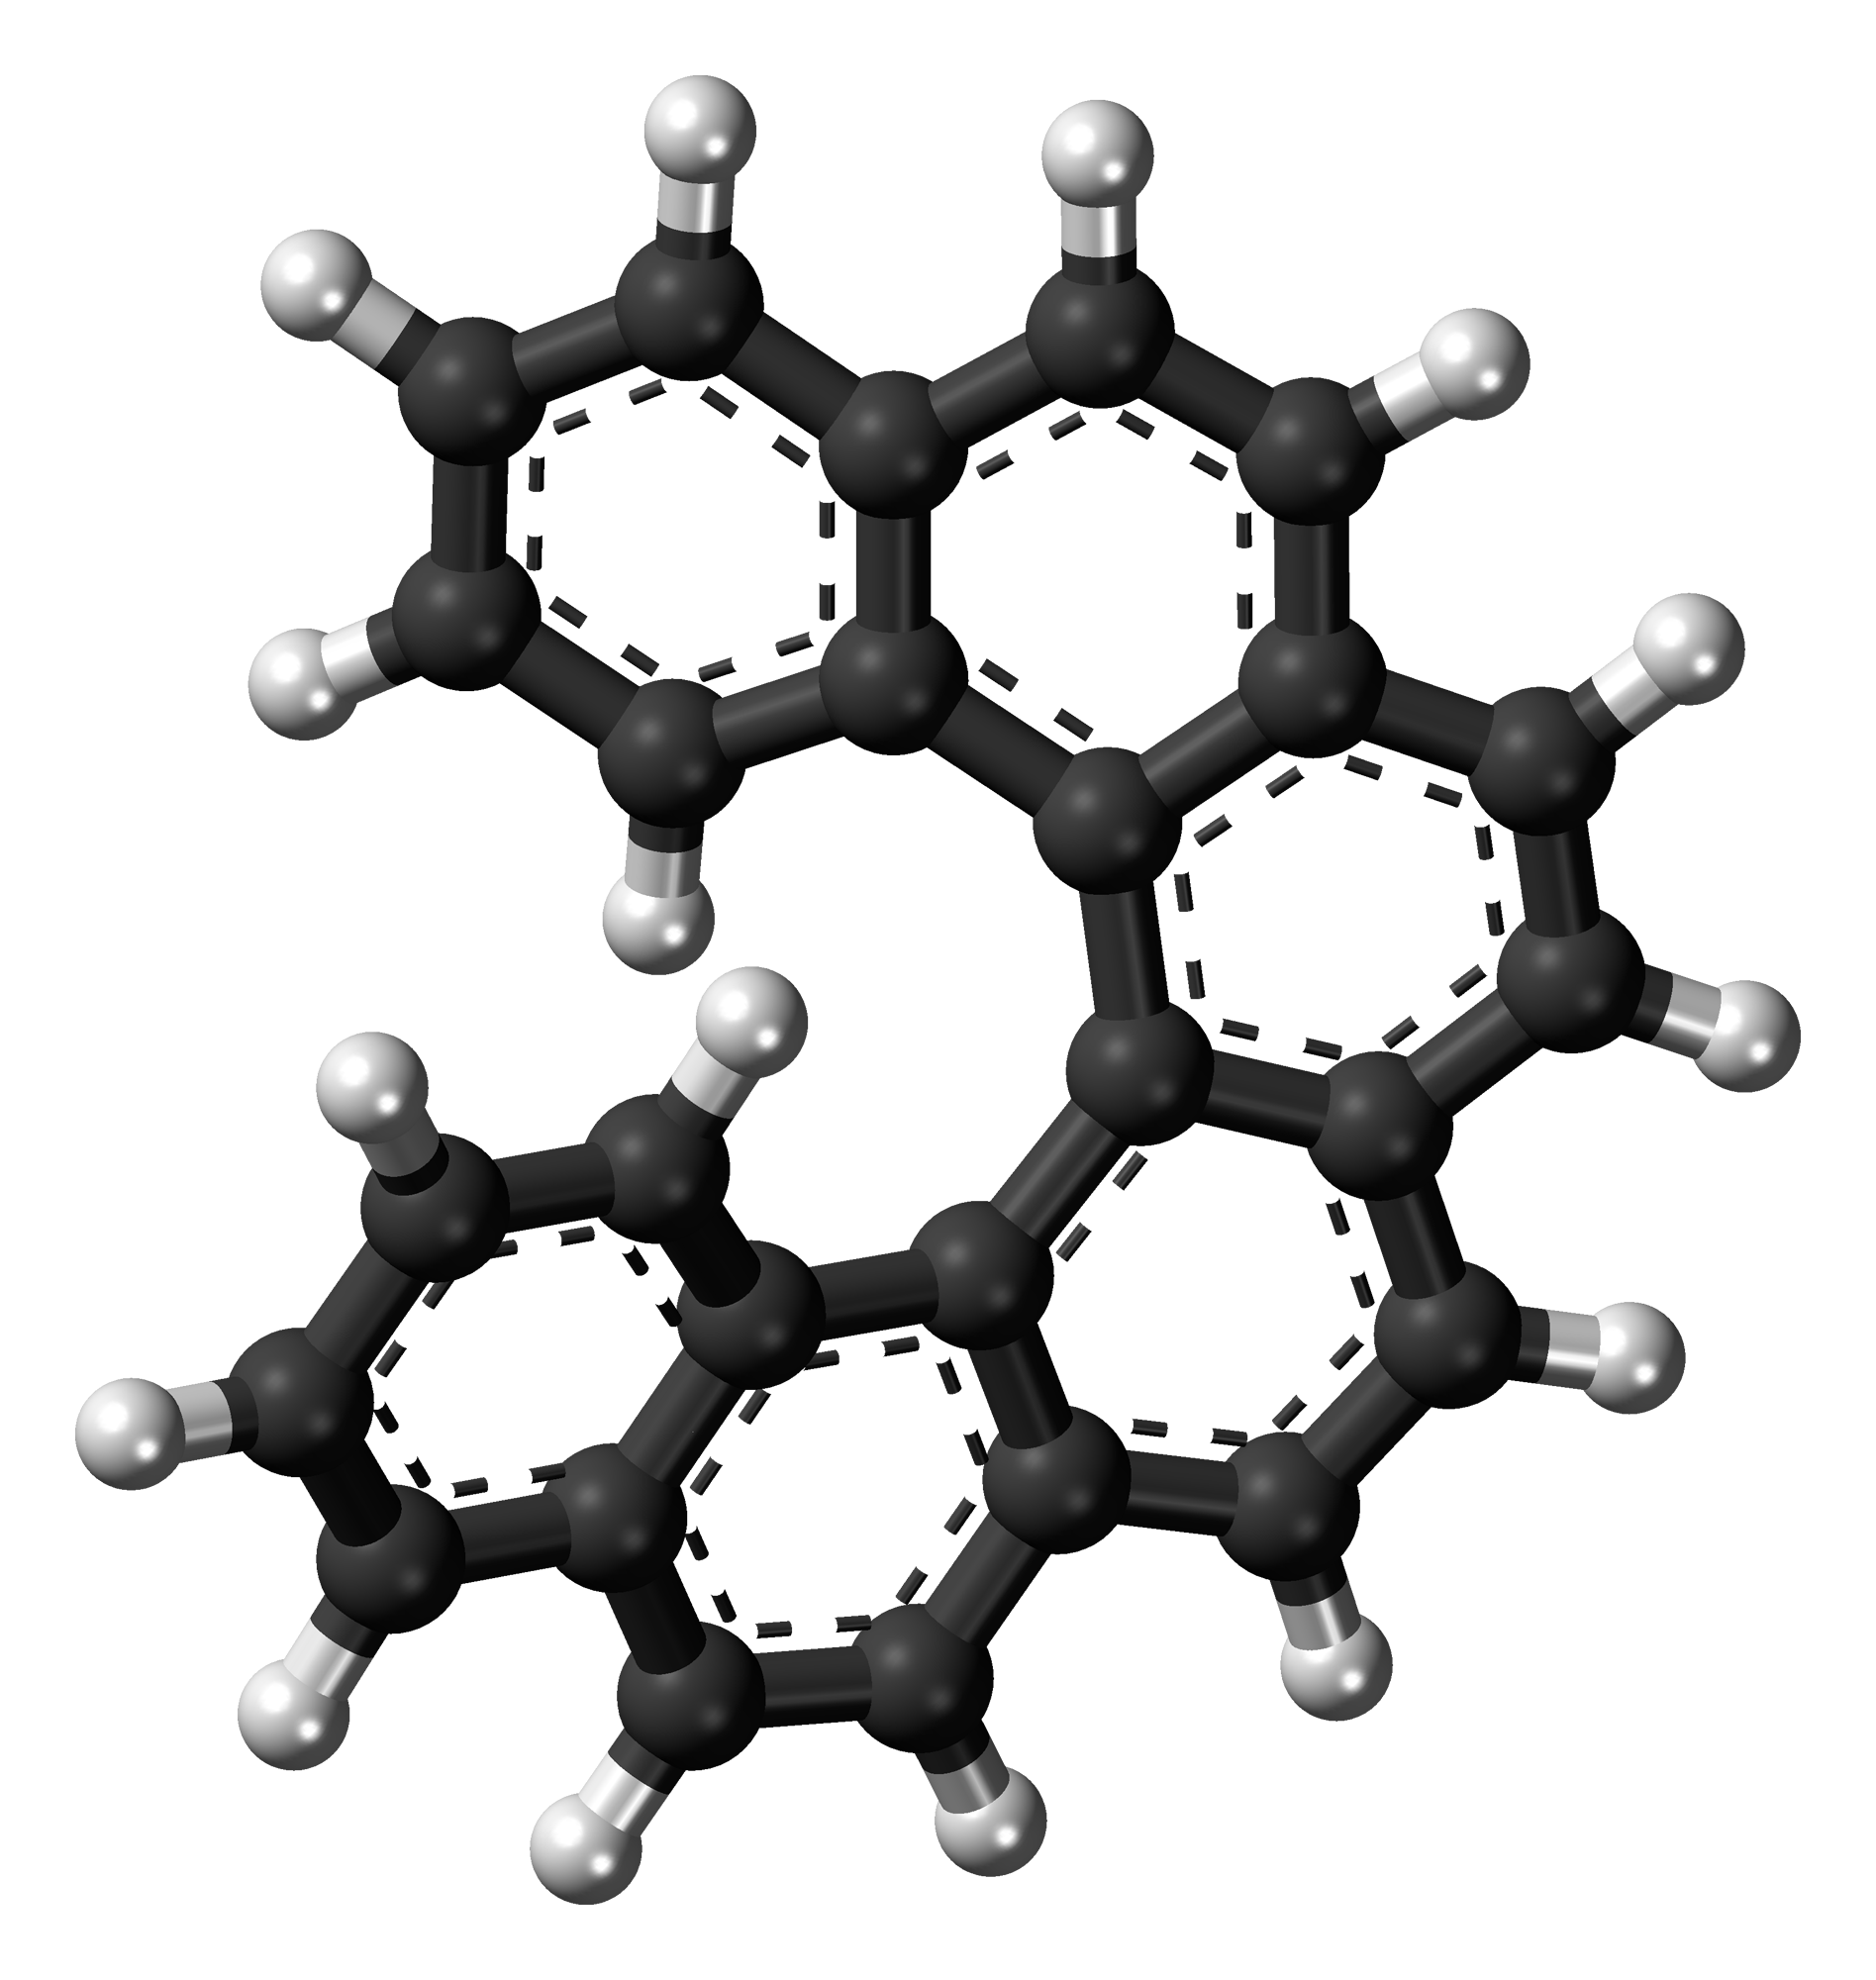
\includegraphics[height=.7\textheight]{img/Hexahelicene-3D-balls.png}
			\end{figure}
		\end{column}
	\end{columns}
	Enantiomery hexahelicenu.\footnote[frame]{Zdroj: \href{https://commons.wikimedia.org/wiki/File:Hexahelicene-3D-balls.png}{Jynto/Commons}}
}

\frame{
	\frametitle{}
	\begin{itemize}
		\item Chirálním centrem nemusí být jen uhlík, ale i např. dusík, síra, kovy, apod.
	\end{itemize}

	\begin{figure}
		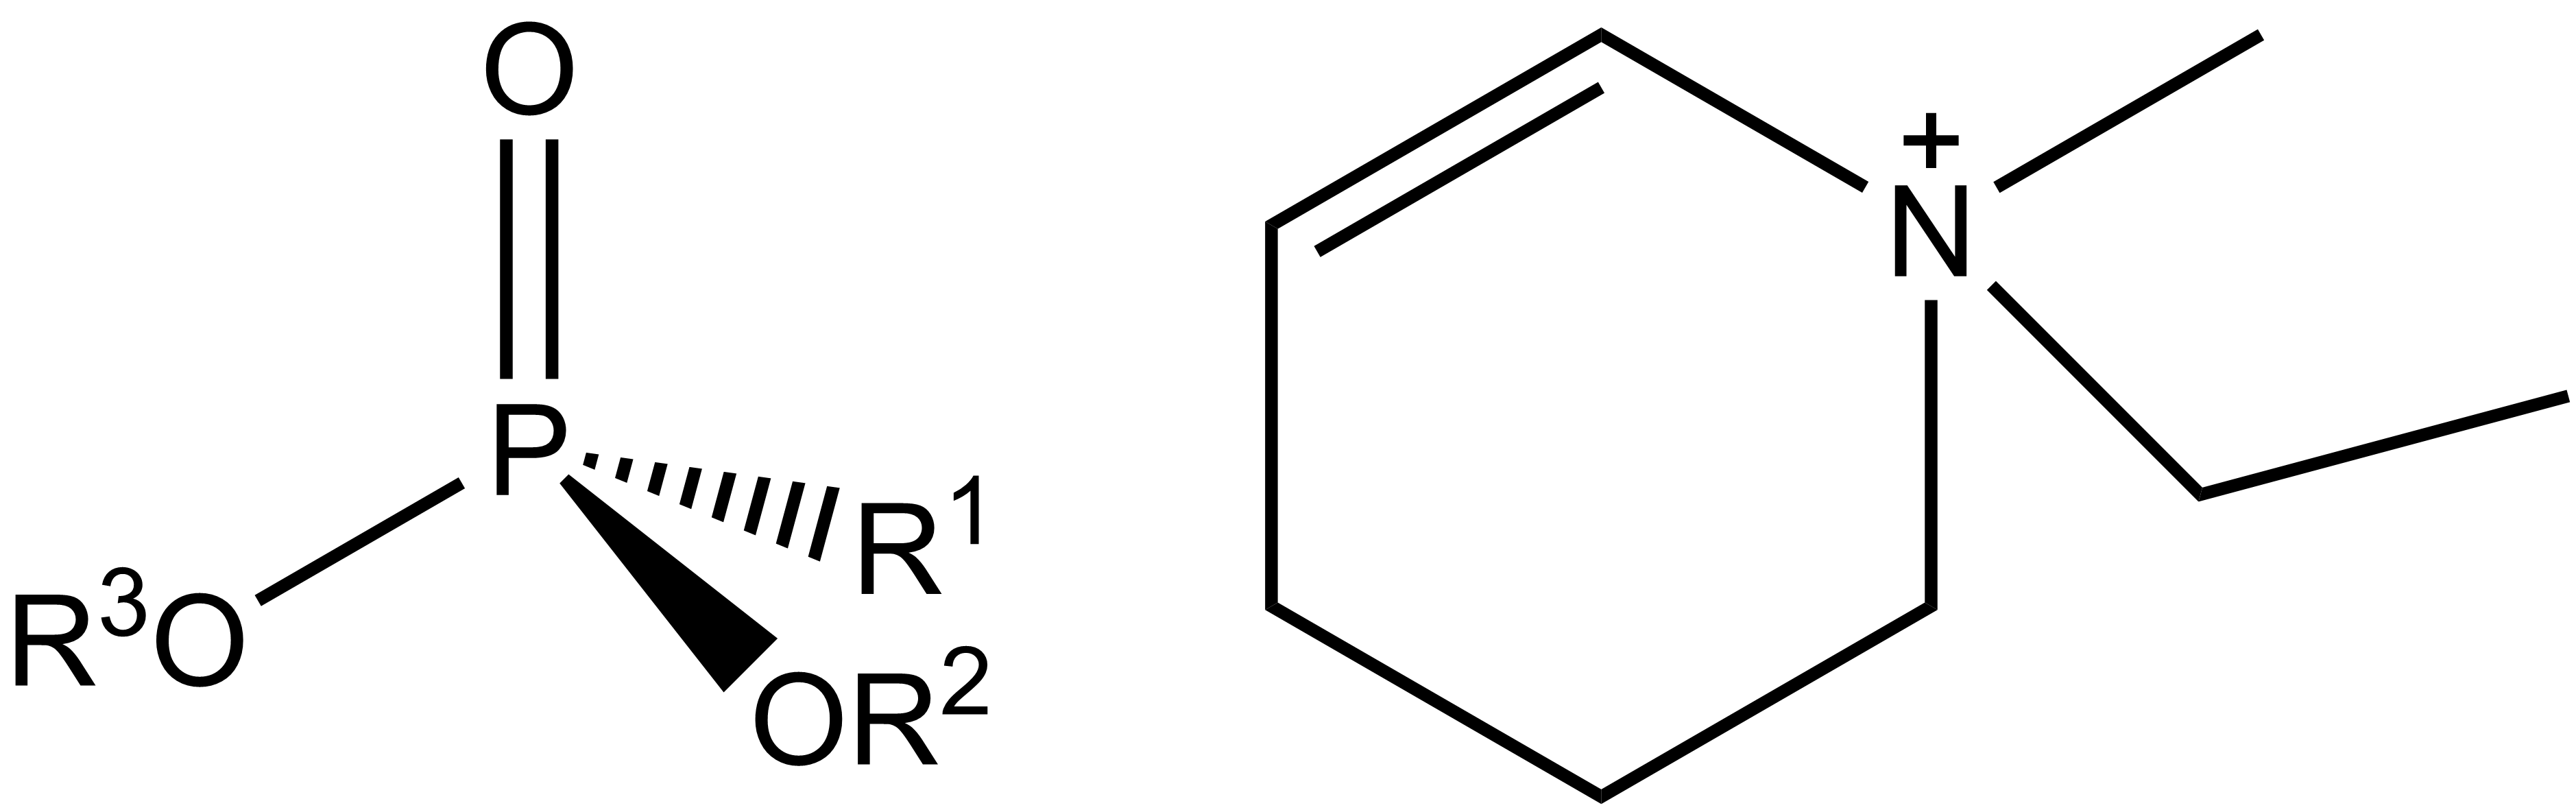
\includegraphics[width=\textwidth]{img/chirality-P-N.png}
		\caption*{Ukázka neuhlíkových chirálních center.}
	\end{figure}
}

\frame{
	\frametitle{}
	\begin{figure}
		
\includegraphics[width=\textwidth]{img/Co-acac-3.png}
		\caption*{Enantiomery acetylacetonátu kobaltitého.\footnote[frame]{Zdroj: \href{https://commons.wikimedia.org/wiki/File:Co(acac)3.png}{Smokefoot/Commons}}}
	\end{figure}
}

\section{Izomerie koordinačních sloučenin}
\frame{
	\frametitle{}

	a) Ligand se koordinuje k centrálnímu atomu různými donorovými atomy. Jev se nazývá \textbf{vazebná izomerie} a izomery rozlišujeme rozdílnými názvy ligandů
	\vspace{5mm}
	\\
	\begin{tabular}{llll}
		\ce{-NO2} & nitro & \ce{-ONO} & nitrito \\
		\ce{-SCN} & thiokyanato & \ce{-NCS} & isothiokyanato \\
		\ce{-SeCN} & selenokyanato & \ce{-NCSe} & isoselenokyanato \\
	\end{tabular}
	\\
	\vspace{10mm}
	b) Koordinují se izomerní ligandy za vzniku \textbf{polohových izomerů}. I tento případ se vystihne rozdílným názvem ligandů
	\vspace{5mm}
	\\
	\begin{tabular}{ll}
		\textcolor{red}{H$_2$N}CH$_2$CH(\textcolor{red}{NH$_2$})CH$_3$ & 1,2-diaminopropan \\
		CH$_3$\textcolor{red}{NH}CH$_2$CH$_2$\textcolor{red}{NH$_2$} & N-methylethylendiamin \\
	\end{tabular}
}

\frame{
	\frametitle{}
	c) Komplex má zaměněny ionty v koordinační a iontové sféře. Tuto situaci, nazývanou \textbf{ionizační izomerie}, řeší název komplexu
	\\
	\vspace{1cm}
	\begin{tabular}{ll}
		\ce{[Co(NH3)5SO4]Br} & bromid pentaammin-sulfatokobaltitý \\
		\ce{[Co(NH3)5Br]SO4} & síran pentaammin-bromokobaltitý  \\
	\end{tabular}
	\vspace{1cm}
	\\
	d) U koordinačních sloučenin s komplexním kationtem i aniontem se může měnit rozdělení ligandů mezi koordinačními sférami obou centrálních atomů (\textbf{koordinační izomerie}) \\
	\vspace{1cm}
	\begin{tabular}{ll}
		\ce{[Pt(NH3)4][CuCl4]} & tetrachloroměďnatan tetramminplatnatý \\
		\ce{[Cu(NH3)4][PtCl4]} & tetrachloroplatnatan tetraamminměďnatý \\
	\end{tabular}
}

\frame{
	\frametitle{}

	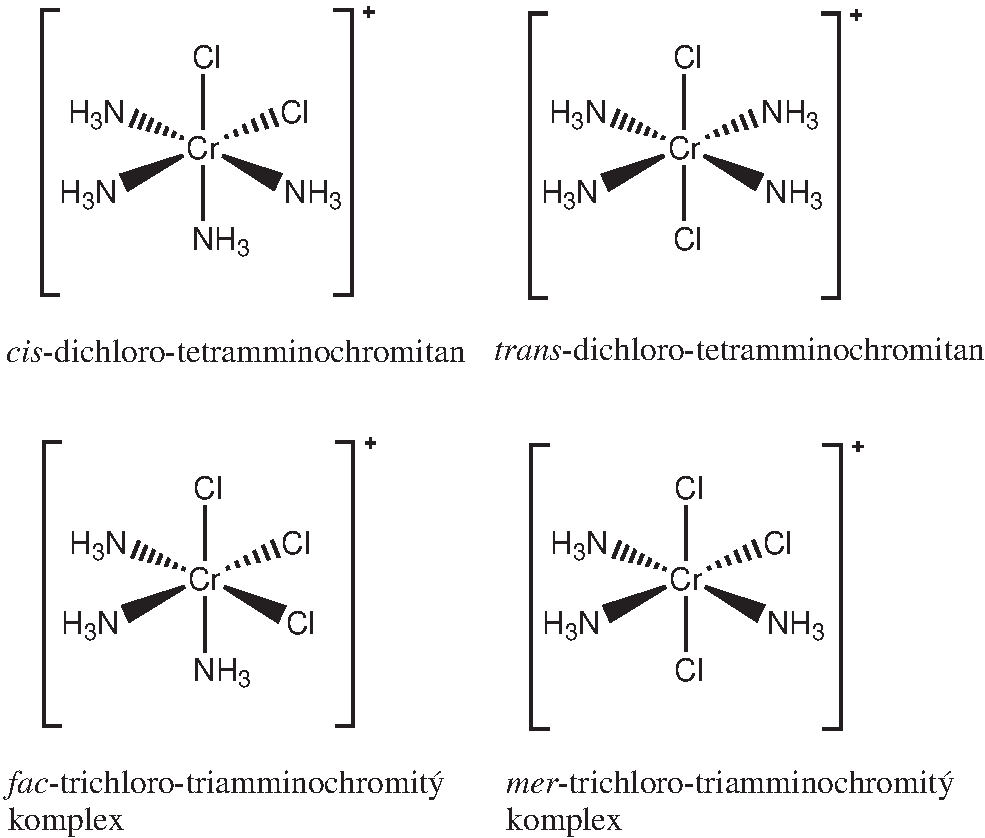
\includegraphics[keepaspectratio,width=100mm]{img/izomery.pdf}
}

\end{document}